\documentclass[a4paper,10pt]{article}
\usepackage[utf8]{inputenc}
\usepackage{verbatim} %for å inkludere filer med tegn LaTeX ikke liker
\usepackage[document]{ragged2e}
\bibliographystyle{plain}
\usepackage{amsmath}
\usepackage{mathtools}
\usepackage[pdftex]{graphicx}
\usepackage{textcomp}
\usepackage{float}
\usepackage{hyperref}
\usepackage[top=0.6in, bottom=0.8in, left=0.9in, right=0.7in]{geometry}
\usepackage{listings}
\usepackage{color}
\usepackage{tikz}
\usepackage{booktabs} 

\begin{document}

\definecolor{codegreen}{rgb}{0,0.6,0}
\definecolor{codegray}{rgb}{0.5,0.5,0.5}
\definecolor{codepurple}{rgb}{0.58,0,0.82}
\definecolor{backcolour}{rgb}{0.95,0.95,0.92}
 
\lstdefinestyle{mystyle}{
    backgroundcolor=\color{backcolour},   
    commentstyle=\color{codegreen},
    keywordstyle=\color{magenta},
    numberstyle=\tiny\color{codegray},
    stringstyle=\color{codepurple},
    basicstyle=\footnotesize,
    breakatwhitespace=false,         
    breaklines=true,                 
    captionpos=b,                    
    keepspaces=true,                 
    numbers=left,                    
    numbersep=5pt,                  
    showspaces=false,                
    showstringspaces=false,
    showtabs=false,                  
    tabsize=2
}
 
\lstset{style=mystyle}

\section*{Problem 33: Double boundary layer}
\subsection*{a)}
\begin{align}
\epsilon y'' - x^2 y' - y = 0 \qquad ; \qquad y(0) = y(1) = 1 \label{org.eq.}
\end{align}
where: $\epsilon \rightarrow 0^+$\\
To find the outer solution we can solve the unperturbed equation where $\epsilon = 0$.
\begin{align}
&-x^2 y_0' - y_0 = 0 \qquad \Rightarrow \qquad \frac{y_0'}{y_0}= -\frac{1}{x^2}
\qquad \Rightarrow \qquad ln(y) = \frac{1}{x} + C \nonumber \\
&\Rightarrow y_0 = Ce^{\frac{1}{x}} \label{out.sol.}
\end{align}

By letting $\epsilon=0$, eq.(\ref{org.eq.}) will have one less term and we can see that that the boundary conditions are not fulfilled, so $-x^2y_0' - y_0 = 0$ cannot be a valid leading order approximation. Also $\epsilon y''$ cannot be small everywhere, and it's presumably important close to $x=0$, so we must have a boundary layer there. We also have that \[ \lim_{x \to 0} y_0 = \infty \qquad \text{if} \qquad C \neq 0 \] so C must then be zero and $y_0 = 0$.\\

\subsection*{b)} To find the inner solution, we must determine the boundary layer thickness $\delta$. If $\epsilon y''$ is not small, then $\epsilon$ shouldn't be there, meaning that we should rescale the the eq.(\ref{org.eq.}) so $\epsilon$ is on the right place.\\
We can do this by introducing $\xi_L = \frac{x}{\delta_L}\quad \Rightarrow \quad x^2 = \xi_L^2 \delta_L^2$, for the \textbf{left boundary layer}.\\
\begin{align*}
\Rightarrow \frac{\epsilon}{\delta_L^2} \frac{d^2 y}{d \xi_L^2} 
&- \frac{x^2}{\delta_L} \frac{d y}{d \xi_L} - y = 0\\\\
\frac{\epsilon}{\delta_L^2} \frac{d^2 y}{d \xi_L^2} 
&- \frac{\xi_L^2 \delta_L^2}{\delta_L} \frac{d y}{d \xi_L} - y = 0\\\\
\frac{\epsilon}{\delta_L^2} \frac{d^2 y}{d \xi_L^2} 
&- \xi_L^2 \delta_L \frac{d y}{d \xi_L} - y = 0
\end{align*}
\hspace{6.8cm} \textcircled{1} \hspace{9mm} \textcircled{2} \hspace{7mm} \textcircled{3}\\
\vspace{2mm}
We can see that \textcircled{2} is not really an option for dominant balance, because whatever $\delta$ is then $\xi_L^2 \delta_L$ is small, so \textcircled{2} is sub-dominant.\\
\vspace{4mm}
\hspace{5.6cm}\textcircled{1} $\sim$ \textcircled{3}
$\quad \Rightarrow \quad \frac{\epsilon}{\delta_L^2}-1=0 \quad \Rightarrow \quad \delta_L = \sqrt{\epsilon}$\\

\begin{align}
\Rightarrow \frac{d^2 y_L}{d \xi_L^2} - y_L = 0 \label{left.eq.}
\end{align}

\begin{align}
y_L = A_L e^{-\xi_L} + B_L e^{\xi_L} \nonumber
\end{align}
\vspace{2mm}
The second term in the solution must be rejected since it grows exponentially out of the boundary layer.\\
We have that $y(0) = 1$
\begin{align}
y_L = A_L e^{-\xi_L} \quad \Rightarrow \quad y_L(0) = A_L = 1 \quad \Rightarrow \quad y_L = e^{-\xi_L} \label{inner sol.}
\end{align}
\vspace{2mm}
But again we cannot fulfill both boundary conditions, so we need a boundary layer at $x = 1$ as well.\\ 
\newpage
\textbf{Right boundary layer:}\\
\begin{align}
\xi_R = \frac{1-x}{\delta_R} \quad \Rightarrow \quad \frac{\epsilon}{\delta_R^2} \frac{d^2 y}{d \xi_R^2} + \frac{1}{\delta_R}(1-\delta_R \xi_R)^2 \frac{d y}{d \xi_R} - y = 0 \nonumber
\end{align}
\hspace{7.5cm} \textcircled{1} \hspace{16mm} \textcircled{2} \hspace{15mm} \textcircled{3}\\
\vspace{4mm}
\hspace{5.6cm}\textcircled{1} $\sim$ \textcircled{2}
$\quad \Rightarrow \quad \frac{\epsilon}{\delta_R^2}=\frac{1}{\delta_R} \quad \Rightarrow \quad \delta_R = \epsilon$
\begin{align}
\frac{\delta_R}{\delta_R^2} \frac{d^2 y}{d \xi_R^2} + \frac{1}{\delta_R}(1-\delta_R \xi_R)^2 \frac{d y}{d \xi_R}=0 \nonumber
\end{align}
Where $(1 - 2 \epsilon \xi_R + \epsilon^2 \xi_R^2) \simeq 1$ since $\epsilon \ll 1$
\begin{align}
\Rightarrow \quad \frac{d^2 y_R}{d \xi_R^2} + \frac{d y_R}{d \xi_R} = 0 \label{Right eq.}
\end{align}
We assume the solution will be proportinal to $e^{\lambda \xi}$ for some constant $\lambda$. Then we substitute this solution into eq.:\ref{Right eq.}:
\begin{align}
&\Rightarrow \quad \frac{d^2}{d \xi_R^2}(e^{\lambda \xi}) + \frac{d}{d \xi_R}(e^{\lambda \xi}) = 0 \nonumber \\
&\Rightarrow \qquad \lambda^2 e^{\lambda \xi} + \lambda e^{\lambda \xi}=0 \nonumber \quad \Rightarrow \quad (\lambda^2 + \lambda)e^{\lambda x}=0 \nonumber \quad \Rightarrow \quad \lambda(1+\lambda)=0 \quad \Rightarrow \quad \lambda=-1 \quad \text{or} \quad \lambda = 0 \nonumber\\
&\Rightarrow \quad y_R = A_R e^{-\xi_R} + B_R \quad , \quad y_R(0)=1 \quad \Rightarrow \quad y_R = A_R e^{-\xi_R} + (1-A_R) \label{Right sol.}
\end{align}

\section*{c)}
We now need to find the unified solution by matching.

\[
\begin{rcases}
\lim_{x \to 0} Ce^{\frac{1}{x}} \quad \Rightarrow \quad C=0 \\
\lim_{\xi_L \to \infty} e^{-\xi_L} = 0
\end{rcases}
\quad
\begin{array}{r@{\;}l} % make space to RHS of \in and = symbols equal to that used for mathrel items
\Rightarrow \quad y_{match,left} = 0 
\end{array}
\]
\vspace{8mm}
\[
\begin{rcases}
\lim_{x \to 1} Ce^{\frac{1}{x}}=0 \quad \text{since} \quad C=0 \\
\lim_{\xi_R \to \infty} (1-A_R)+A_R e^{-\xi_R} = 1-A_R\\
\Rightarrow \quad A_R=1
\end{rcases}
\quad
\begin{array}{r@{\;}l} % make space to RHS of \in and = symbols equal to that used for mathrel items
\Rightarrow \quad y_{match,Right} = 0 
\end{array}
\]

\begin{align}
y_{unified} = y_R + y_L - y_{match,Right} - y_{match,left} = e^{-\xi_R} + e^{-\xi_L} = e^{\frac{-1+x}{\epsilon}} + e^{\frac{-x}{\sqrt{\epsilon}}}
\end{align}

\begin{figure}[H]
    \centering
    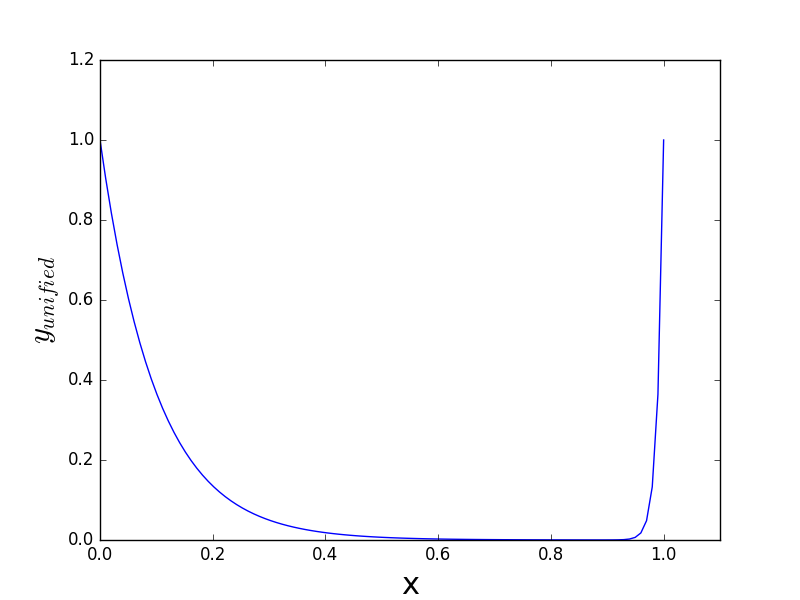
\includegraphics[width=12cm, height=7cm]{figure_1.png}
    \caption{Double boundary layer solution}
    \label{fig:1}
\end{figure}

\newpage

\section*{Problem 50: The perturbed satellite orbit}
We seek an approximate solution to:
\begin{align}
(1+\epsilon z)^3\frac{d^z}{d \tau^2} + z = 0 \quad , \quad z(0) = 0 \quad , \quad \frac{d z}{d \tau}(0) = 1
\end{align}
by a straightforward perturbation expansion of z in $\epsilon$.
\subsection*{a)}
We want to find the first two terms in a series for z.\\
We can try with a solution of the form: 
$$z(\tau) = z_0(\tau) + \epsilon z_1(\tau) + \epsilon^2 z_2(\tau) + ... $$

I choose to do the perturbation expansion for z up to order $\epsilon^2$, because even though I do not need it for the first part of the problem, I will need it for the second part of the problem, where I have to check if the expansion breaks down at order $\epsilon^2$.

\begin{align*}
&(1+3\epsilon(z_0 + \epsilon z_1+...)+3\epsilon^2(z_0+...)^2)(z_0''+\epsilon z_1'' + \epsilon^2 z_2'')+z_0 + \epsilon z_1 + \epsilon^2 z_2 = 0\\[2mm]
&(1+3\epsilon z_0 + 3 \epsilon^2 z_1 +3\epsilon^2 z_0^2)(z_0''+\epsilon z_1'' + \epsilon^2 z_2'')+z_0 + \epsilon z_1 + \epsilon^2 z_2 = 0\\[2mm]
&z_0'' + \epsilon z_1'' + \epsilon^2 z_2'' + 3 \epsilon z_0 z_0'' + 3 \epsilon^2 z_0 z_1'' + 3 \epsilon^2 z_0'' z_1 + 3 \epsilon^2 z_0^2 z_0'' + z_0 + \epsilon z_1 + \epsilon^2 z_2 = 0\\
\end{align*}

For the initial conditions we get:
\begin{align*}
&z_0(0) + \epsilon z_1(0) + \epsilon^2 z_2(0) = 0\\
\Rightarrow \quad &z_0(0) = 0,
\quad z_1(0) = 0,
\quad z_2(0) = 0\\\\
&z_0'(0) + \epsilon z_1'(0) + \epsilon^2 z_2'(0) = 1\\
\Rightarrow \quad &z_0'(0) = 1,
\quad z_1'(0) = 0,
\quad z_2'(0) = 0\\
\end{align*}
We then have to collect the terms for $\epsilon^0$ and $\epsilon^1$:

\begin{align}
\epsilon^0 &: z_0 + z_0 = 0 \quad \Rightarrow \quad 
z_0 = A_0 \sin(\tau) + B_0 \cos(\tau) \label{z0_eq}\\
&z_0(0) = 0 \quad \Rightarrow \quad B_0 = 0 \quad \Rightarrow \quad z_0 = A_0 \sin(\tau) \nonumber \\
&z_0'(0) = 1 \quad \Rightarrow \quad A_0 = 1 \nonumber \\ 
\Rightarrow \quad &z_0=\sin(\tau) \label{z0_sol}\\[6mm]
\epsilon^1 &: z_1'' + 3z_0 z_0'' + z_1 = 0 \nonumber \\
\Rightarrow \quad &z_1'' + z_1 = -3 z_0 z_0'' = 3 \sin^2(\tau) = \frac{3}{2}(1-\cos(2 \tau)) = \frac{3}{2} - \frac{3}{2} \cos(2 \tau) \label{z1_eq}\\
&z_1(\tau) = z_1^P + z_1^H = z_1^P + A_1 \cos(\tau) + B_1 \sin(\tau) \nonumber
\end{align}

Where the particular solution $z_1^P$, must be of the form:\\
\begin{align}
&z_1^P = a_1 - b_1 \cos(2 \tau) \nonumber\\
\end{align}

We substitute for this solution into eq.(\ref{z1_eq}) and get:

\begin{align}
&4 b_1 \cos(2 \tau) + a_1 - b_1 cos(2 \tau) = \frac{3}{2} - \frac{3}{2} \cos (2 \tau) \quad \Rightarrow \quad a_1 = \frac{3}{2} \nonumber \\
\Rightarrow \quad &3b_1 \cos(2 \tau) = - \frac{3}{2} \cos(2 \tau) \quad \Rightarrow \quad b_1 = -\frac{1}{2} \nonumber \\
&z_1^P = \frac{3}{2} + \frac{1}{2}\cos(2 \tau) \nonumber\\
\Rightarrow \quad &z_1 = \frac{3}{2} + \frac{1}{2}\cos(2 \tau) + A_1 \cos(\tau) + B_1 \sin(\tau) \nonumber \\
&z_1(0) = \frac{3}{2} + \frac{1}{2} + A_1 = 0 \quad 
\Rightarrow \quad A_1 = -2 \nonumber \\
&z_1'(0) = -\sin(0) + 2\sin(0) + B_1 \cos(0) = B_1 = 0 \nonumber \\\nonumber\\
\Rightarrow \quad &z_1 = \frac{3}{2} + \frac{1}{2} \cos(2 \tau) - 2 \cos(\tau) \label{z1_sol}
\end{align}
The first two terms in a series for z are then:

\begin{align}
z = \underbrace{\sin (\tau)}_\text{$z_0(\tau)$} + \underbrace{\frac{3 \epsilon}{2} + \frac{\epsilon}{2} \cos(2 \tau) - 2 \epsilon \cos(\tau)}_\text{$\epsilon z_1(\tau)$} \label{z_sol_twoterms}
\end{align}

\subsection*{b)}
To find $z_2$, we need to solve the equation that we will get by collecting all the terms of order $\epsilon^2$ in the perturbation expansion for z.  

\begin{align*}
z_2''+ z_2 &= -3(-z_0 z_1 + 3z_0^3 - z_0 z_1 - z_0^3)\\
&= 6 \sin(\tau) \bigg(\frac{1}{2} \cos(2 \tau) - 2 \cos(\tau) + \frac{3}{2}\bigg) - 6 \sin^3(\tau)\\
&= 3 \sin(\tau) \cos(\tau) - 12 \sin(\tau) \cos(\tau) + 9 \sin(\tau) - 6 sin^3(\tau)\\
\end{align*}
This expression can be rewritten into an expression with only first order sinus terms, using trigonometric formulas:
\begin{align}
z_2''+ z_2 &= -\frac{3}{2} \sin(\tau) + \frac{3}{2} \sin(3 \tau) - 6 \sin (2 \tau) + 9 \sin(\tau) - \frac{9}{2} \sin(\tau) + \frac{3}{2} \sin(3 \tau) \nonumber \\
&= 3 \sin(3 \tau) -6 \sin (2 \tau) + 3 \sin(\tau) \label{z2_eq}\\ \nonumber \\
z_2(\tau) &= z_2^P + z_2^H \nonumber\\\nonumber
\end{align}
We can use the method of undetermined coefficients to find the particular solution, which will be the sum of the particular solutions to:

\begin{align}
z_{2,1}'' + z_{2,1} &= 3 \sin(\tau) &&\Rightarrow \quad z_{2,1}^P= a_2 \tau \cos(\tau) + b_2 \tau \sin(\tau) \label{z21_p} \\
z_{2,2}'' + z_{2,2} &= -6 \sin(2 \tau)  &&\Rightarrow \quad z_{2,2}^P= c_2 \cos(2 \tau) + d_2 \sin(2 \tau) \label{z22_p} \\
z_{2,3}'' + z_{2,3} &= 3 \sin(3 \tau) &&\Rightarrow \quad z_{2,3}^P= e_2 \cos(3 \tau) + f_2 \sin(3 \tau) \label{z23_p} \\\nonumber
\end{align}

We can see from the first part of the particular solution (\ref{z21_p}), that we have non-periodic terms that will grow in time so $\epsilon^2 \tau \gg 1$ and $\epsilon^2 z_2 \gg z_0$. This means that the straightforward perturbation expansion breaks down at order $\epsilon^2$. The remedy to this problem would be the \textbf{Poincaré-Lindstedt method}.\\
\vspace{4mm}
We introduce a rescaled time, set $\sigma = \omega \tau$ and seek a solution of period $2 \pi$ in $\sigma$, so $\omega \tau$ will change by $2 \pi$ for each period.\\
\newpage
The rescaled equation is:

\begin{align}
&\frac{d^2 z}{d \tau^2} = \omega^2 \frac{d^2 z}{d \sigma^2} \quad \Rightarrow \quad \omega^2(1 + \epsilon z)^3 \hspace{1mm} \frac{d^2 z}{d \sigma^2} + z = 0 \label{rescaled_eq}\\
&z(0) = 0 \qquad , \qquad \omega \frac{d z}{d \sigma}(0) = 1 \label{IC}\\ \nonumber \\
&z = z_0 + \epsilon z_1 + \epsilon^2 z_2 \qquad \text{and} \qquad \omega = \omega_0 + \epsilon \omega_1 + \epsilon^2 \omega_2 \nonumber
\end{align}
Since the straightforward perturbation expression worked for the first two terms and we didn't have to use the Poincaré-Lindstedt method for those two terms, we set $\omega_0 = 1$ and $\omega_1 = 0$ so $\mathcal{O}(\epsilon^0)$ and $\mathcal{O}(\epsilon^1)$ remain unaltered.

\begin{align}
(\omega_0 + \epsilon \omega_1 + \epsilon^2 \omega_2)(1+3\epsilon z_0 + 3\epsilon^2 z_1 + 3 \epsilon^2 z_0^2)(z_0'' + \epsilon z_1'' + \epsilon^2 z_2'')+ z_0 + \epsilon z_1 + \epsilon^2 z_2 =0 \nonumber
\end{align}
\begin{align}
\epsilon^2 = z_2'' + z_2 &= -6 z_0^3 + 6 z_0 z_1 -2 \omega_2 z_0'' = -6 z_0^3 + 6 z_0 z_1 + 2 \omega_2 z_0 \nonumber\\
&= 3 \sin(3 \tau) + 3 \sin(\tau) -6 \sin(2 \tau) - 2 \omega_2 \sin(\tau)\nonumber\\
&= 3 \sin(3 \tau) - 6 \sin(2 \tau) + (3 - 2\omega_2) \sin(\tau) \nonumber
\end{align}
$(3 - 2\omega_2)$ must be 0 to avoid secular or non-periodic terms. $\quad \Rightarrow \quad \omega_2 = -\frac{3}{2}$\\[1em]
We have now that: 
\begin{align}
&z_2'' + z_2 = 3 \sin(3 \tau) -6 \sin(2 \tau) \label{PL_z2_eq}\\
&z_2 = z_2^H + z_2^P \quad \text{where} \quad z_2^H = A_2 \sin(\tau) + B_2 \cos(\tau)\nonumber \\
&z_2^P = a_2 \cos(2 \tau) + b_2 \cos(3 \tau) + c_2 \sin(2 \tau) + d_2 \sin(3 \tau) \label{z2p}\\ \nonumber
\end{align}
We then need to substitute (\ref{z2p}) into (\ref{PL_z2_eq}).
\begin{align}
z_2'' = &-4 a_2 \cos(2 \tau) - 9 b_2 \cos(3 \tau) - 4 c_2 \sin(2 \tau) - 9 d_2 \sin(3 \tau) \nonumber \\[2mm]
z_2'' + z_2 = &-4 a_2 \cos(2 \tau) - 9 b_2 \cos(3 \tau) - 4 c_2 \sin(2 \tau) - 9 d_2 \sin(3 \tau) \nonumber \\
&+ a_2 \cos(2 \tau) + b_2 \cos(3 \tau) + c_2 \sin(2 \tau) + d_2 \sin(3 \tau)\nonumber\\
=&-3 a_2 \cos(2 \tau) - 8 b_2 \cos(3 \tau) - 3 c_2 \sin(2 \tau) - 8 d_2 \sin(3 \tau) \nonumber \\
= & \hspace{1mm}3 \sin(3 \tau) -6 \sin(2 \tau) \quad \Rightarrow \quad a_2 = b_2 = 0 \nonumber \\
&\Rightarrow \qquad -3 c_2 = -6 \qquad \Rightarrow \qquad c_2 = 2 \nonumber \\
&\Rightarrow \qquad -8 d_2 = -3 \qquad \Rightarrow \qquad d_2 = -\frac{3}{8} \nonumber \\
&\Rightarrow \qquad z_2^P = 2 \sin(2 \tau) - \frac{3}{8} \sin(3 \tau) \nonumber \\ \nonumber \\
z_2 &= z_2^H + z_2^P = A_2 \sin(\tau) + B_2 \cos(\tau) + 2 \sin(2 \tau) - \frac{3}{8} \sin(3 \tau)\\ \nonumber
\end{align}
The initial conditions will give us the constants $A_2$ and $B_2$.
\begin{align*}
\omega \frac{dz}{d \sigma}(0) = 1 \quad &\Rightarrow \quad (1+\epsilon^2 \omega_2)(z_0'(0) + \epsilon z_1'(0) + \epsilon^2 z_2'(0)) = 1  \\[2mm]
&\Rightarrow  \quad \epsilon^0 : z_0'(0) = 1  \\[2mm]
&\Rightarrow  \quad \epsilon^1 : z_1'(0) = 0  \\[2mm]
&\Rightarrow  \quad \epsilon^2 : z_2'(0) + \omega_2 \\ 
\end{align*}
\newpage
\begin{align*}
z_0'(0) &= 0 \quad \Rightarrow \quad z_2'(0) = -\omega_2 \quad \Rightarrow \quad z_0'(0) = \frac{3}{2} \\
z_2(0) &= B_2 = 0 \quad \Rightarrow \quad z_2 = A_2 \sin(\tau) + 2 \sin(2 \tau) - \frac{3}{8} \sin(3 \tau) \\ 
z_2'(0) &= A_2 \cos(\tau) + 4 \cos(2 \tau) - \frac{9}{8} \sin(3 \tau) = A_2 + 4 = \frac{3}{2} \quad \Rightarrow \quad A_2 = -\frac{5}{2} 
\end{align*}
\begin{align}
z_2 = -\frac{5}{2} \sin(\tau) + 2 \sin(2 \tau) - \frac{3}{8} \sin(3 \tau) \\ \nonumber
\end{align}
Finally we have the full solution to order $\epsilon^2$:
\begin{align}
z &= z_0 + \epsilon z_1 + \epsilon^2 z_2 \nonumber\\[0.7em]
&= \sin(\tau) + \epsilon \bigg( \frac{1}{2} \cos(2 \tau) - 2 \cos(\tau) + \frac{3}{2}\bigg) + \epsilon^2 \bigg(-\frac{3}{8} \sin(3 \tau) + 2 \sin(2 \tau) -\frac{5}{2} \sin(\tau)\bigg) \label{final_solution}
\end{align}
\end{document}